\documentclass[conference]{IEEEtran}
\IEEEoverridecommandlockouts
% The preceding line is only needed to identify funding in the first footnote. If that is unneeded, please comment it out.
\usepackage{cite}
\usepackage{amsmath,amssymb,amsfonts}
\usepackage{algorithmic}
\usepackage{graphicx}
\usepackage{textcomp}
\usepackage{xcolor}
\usepackage{tabularx}
\usepackage{multirow}
\usepackage{graphics} % for pdf, bitmapped graphics files
\usepackage{subfig}
\usepackage{subcaption}
\usepackage{hyperref}
\usepackage{academicons}
\usepackage{xcolor}
\usepackage{listings}
\usepackage{tabularx} % Asegúrate de incluir este paquete

\usepackage{tikz}
\usetikzlibrary{shapes.geometric, arrows}

\usetikzlibrary{shapes.geometric, arrows}

\tikzstyle{startstop} = [rectangle, rounded corners, minimum width=3cm, minimum height=1cm,text centered, draw=black, fill=red!30]
\tikzstyle{process} = [rectangle, minimum width=3cm, minimum height=1cm, text centered, draw=black, fill=blue!30]
\tikzstyle{arrow} = [thick,->,>=stealth]


\def\BibTeX{{\rm B\kern-.05em{\sc i\kern-.025em b}\kern-.08em
		T\kern-.1667em\lower.7ex\hbox{E}\kern-.125emX}}

% Color Enlace
\definecolor{colorEnlace}{RGB}{0, 0, 0}
\hypersetup{
	colorlinks=true,
	linkcolor=colorEnlace,
	citecolor=colorEnlace,
	urlcolor=colorEnlace,
	pdfauthor={Davis Bremdow Salazar Roa},
	pdftitle={Fundamentos de Bioningeniería}
}
\definecolor{mybg}{rgb}{0.97,0.97,0.97}
\definecolor{mygray}{gray}{0.4}
\definecolor{mygreen}{rgb}{0,0.6,0}
\definecolor{myblue}{rgb}{0,0,0.8}
\definecolor{mypurple}{rgb}{0.58,0,0.82}
\definecolor{myred}{rgb}{0.7,0,0}

\lstdefinelanguage{MatlabEnhanced}{
	language=Matlab,
	morekeywords={[2]linspace,plot,title,xlabel,ylabel,legend,grid},
	morekeywords={[3]sin,cos,exp,log,sqrt},
	keywordstyle=\color{myblue}\bfseries,
	keywordstyle=[2]\color{mypurple},
	keywordstyle=[3]\color{myred},
	commentstyle=\color{mygreen}\itshape,
	stringstyle=\color{mygray},
	morecomment=[l]%
}

\lstset{
	language=MatlabEnhanced,
	backgroundcolor=\color{mybg},
	frame=single,
	basicstyle=\ttfamily\small,
	showstringspaces=false,
	numbers=none,              %
	xleftmargin=0pt,           %
	framexleftmargin=0pt,      
	framexrightmargin=0pt,
	framextopmargin=2pt,
	framexbottommargin=2pt,
	breaklines=true,
	tabsize=1,
}

% Control 
\usepackage{amsmath}
\begin{document}
	
	\title{Electrofisiología en la membrana del Calamar}
	\author{
		\makebox[\textwidth][c]{\large\textbf{Universidad Nacional de San Antonio Abad del Cusco}}\\
		\makebox[\textwidth][c]{\normalsize\textit{Escuela profesional de Ingeniería Electrónica}}\\
		\makebox[\textwidth][c]{\normalsize\textit{Fundamentos de Bioingenieria}}\\
		\and
		\IEEEauthorblockN{Ing. Luis Jimenez Troncoso}
		\IEEEauthorblockA{Ingeniero Electrónico \\
			Cusco, Perú \\
			luis.jimenez@unsaac.edu.pe}
		\and
		\IEEEauthorblockN{Davis Bremdow Salazar Roa - 200353}
		\IEEEauthorblockA{Estudiante de Ingeniería Electrónica \\
			Cusco, Perú \\
			200353@unsaac.edu.pe
		}
	}
	
	\maketitle
	\begin{abstract}
		
	\end{abstract}
	
	\begin{IEEEkeywords}
		
	\end{IEEEkeywords}
	
	% Contenido del documento
	\section{Estimación del tiempo de respuesta de la membrana celular del calamar}
	
	En la pregunta 5, se obtener el tiempo de respuesta en el cual ocurre la segunda estimulación u obtención del voltaje de membrana positivo (despolarización) para una corriente de excitación (pulso) de $I_i = 20\mu A$ con una duración de 20ms y la cual es adecuada respecto a magnitud debido a que mediante el modelo estudiado previamente tan solo es necesario un nivel de corriente de excitación (pulso) $I_i = 6\mu A$.
	
	Luego para determinar el tiempo en el cual se obtiene una segunda respuesta se modifico el sub-sistema \textbf{pulso de corriente} en especifico los tiempos de inicio para las señales escalón como variables de entorno, para su manipulación desde el script en MATLAB, este cambio se aprecia en la figura \ref{fig:tiemposescalon}.
	
	\begin{figure}[h]
		\centering
		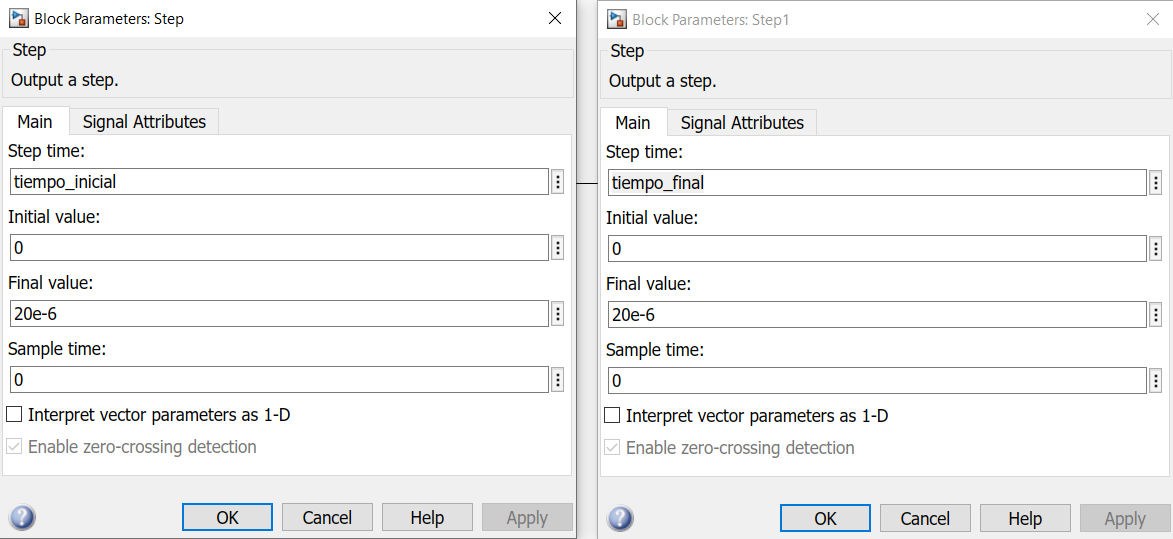
\includegraphics[width=0.5\textwidth]{media/tiempos_escalon}
		\caption{Tiempo de Inicio como variable}
		\label{fig:tiemposescalon}
	\end{figure}
	
	Por otro lado para poder modificar la variable tiempo, se realizo la creación de un script en MATLAB en el cual se definieron los parámetros $tiempo_inicial$ y $tiempo_final$ dentro de un bucle iterativo para poder modificar su valor respecto al tiempo.
	
	Finalmente para determinar un voltaje de membrana umbral se determino una condicional la cual evalúa el valor máximo de la señal de respuesta del modelo, mediante el empleo del vector Y obtenido a partir de la invocación del archivo simulink $MEMBRANA_CALAMAR_GIGANTE_2B$, el código MATLAB para este procedimiento se muestra en el bloque \ref{lst-matlab}
	
	\begin{lstlisting}[numbers=none, caption={Variación del tiempo de respuesta de la membrana Axon de calamar}, label=lst-matlab]
		clc, clear, close all;
		j = 1;
		t_accion = [];
		potencial = [];
		
		for i = 1 : 15 
		% Determinar la cantidad de pulsos espacios 2ms
			tiempo_inicial = 0 + i*4e-3;
			tiempo_final = tiempo_inicial + 2e-3;
			[t, X, Y] = sim("MEMBRANA_CALAMAR_GIGANTE_2B");
			if ( max(Y(:, 1)) > 0)
				t_accion(j) = t(tiempo_inicial*1000);
				potencial(j) = max( Y(:, 1) );
				j = j + 1;
			end
		end
		
		plot(t_accion*1000, potencial*1000);
		title("Tiempo de respuesta a un impulso en la membrana del calamar");
		xlabel("Tiempo [ms]");
		ylabel("Potencial [mV]");
	\end{lstlisting}
	
	Para la obtención de resultados se definieron 2 vectores para almacenar el tiempo y voltaje cuando el potencial de membrana superaba los $0 mV$ y para acceder al tiempo en el cual ocurren estos procesos, se accedió al vector tiempo $t$ obtenido a partir del modelo en simulink, estos resultados se graficaron en una figura resultante que se muestra en \ref{fig:tiempo-respuesta-pulso}
	
	Siendo así que los pulsos ocurren en:
	
	\begin{itemize}
		\item Primer pulso: $0.09 [ms]$ - Potencial de $48.8809 [mV]$
		\item Segundo pulso: $0.21 [ms]$ - Potencial de $48.8911 [mV]$
	\end{itemize}
	
	\newpage

	\begin{figure}[h]
		\centering
		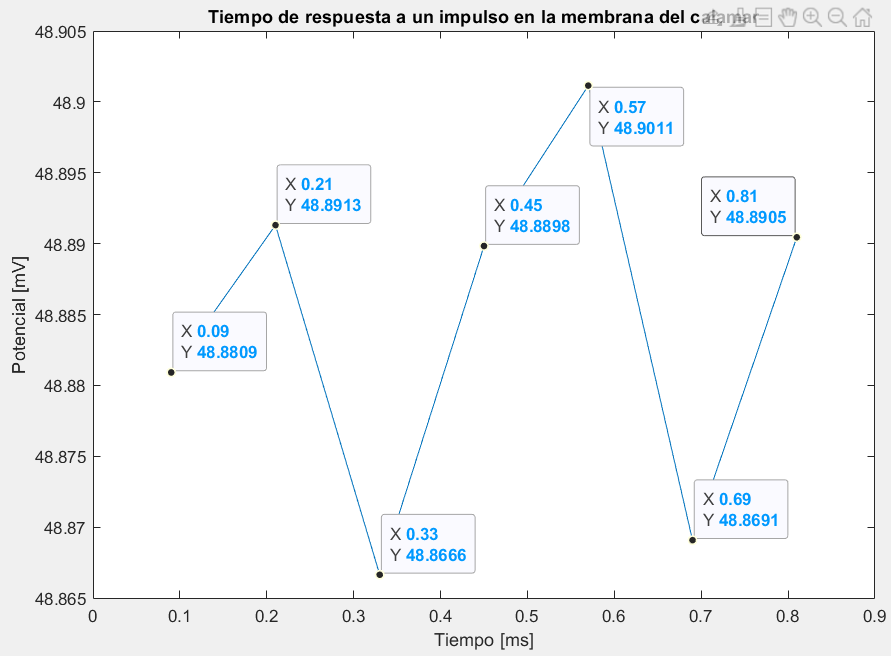
\includegraphics[width=0.5\textwidth]{media/tiempo-respuesta-pulso}
		\caption{Tiempos de respuesta de la membrana frente a la fuente de excitación de 20uA}
		\label{fig:tiempo-respuesta-pulso}
	\end{figure}
	
	
	
	\bibliographystyle{IEEEtran}
	\bibliography{biblio}
\end{document}